\documentclass[11pt,letterpaper]{article}
\usepackage[lmargin=1in,rmargin=1in,tmargin=1in,bmargin=1in]{geometry}
\usepackage{../style/homework}
\usepackage{../style/commands}
\setbool{quotetype}{true} % True: Side; False: Under
\setbool{hideans}{false} % Student: True; Instructor: False

% -------------------
% Content
% -------------------
\begin{document}

\homework{7: Due 10/17}{The irreducible price of learning is realizing that you do not know.}{James Baldwin}

% Problem 1
\problem{10} Do you think a person's height is a function of time? Do you think a person's salary is a function of their body temperature? For each, explain why or why not. \



\newpage



% Problem 2
\problem{10} Determine if the relations $f(x)$ and $g(x)$ shown below are functions. Explain why or why not. If the relation is a function, compute the functions value at $x= -4.1$. 
	\[
	\begin{aligned}
	f(x)&= 198.3 - 17.3x \\[0.3cm]
	g(x)&= 4x^2 + 16.1x - 10.3
	\end{aligned}
	\]



\newpage



 % Problem 3
\problem{10} Plot the function $f(x):= \frac{1}{2}x - 5$, being as accurate as possible. 
	\[
	\fbox{
	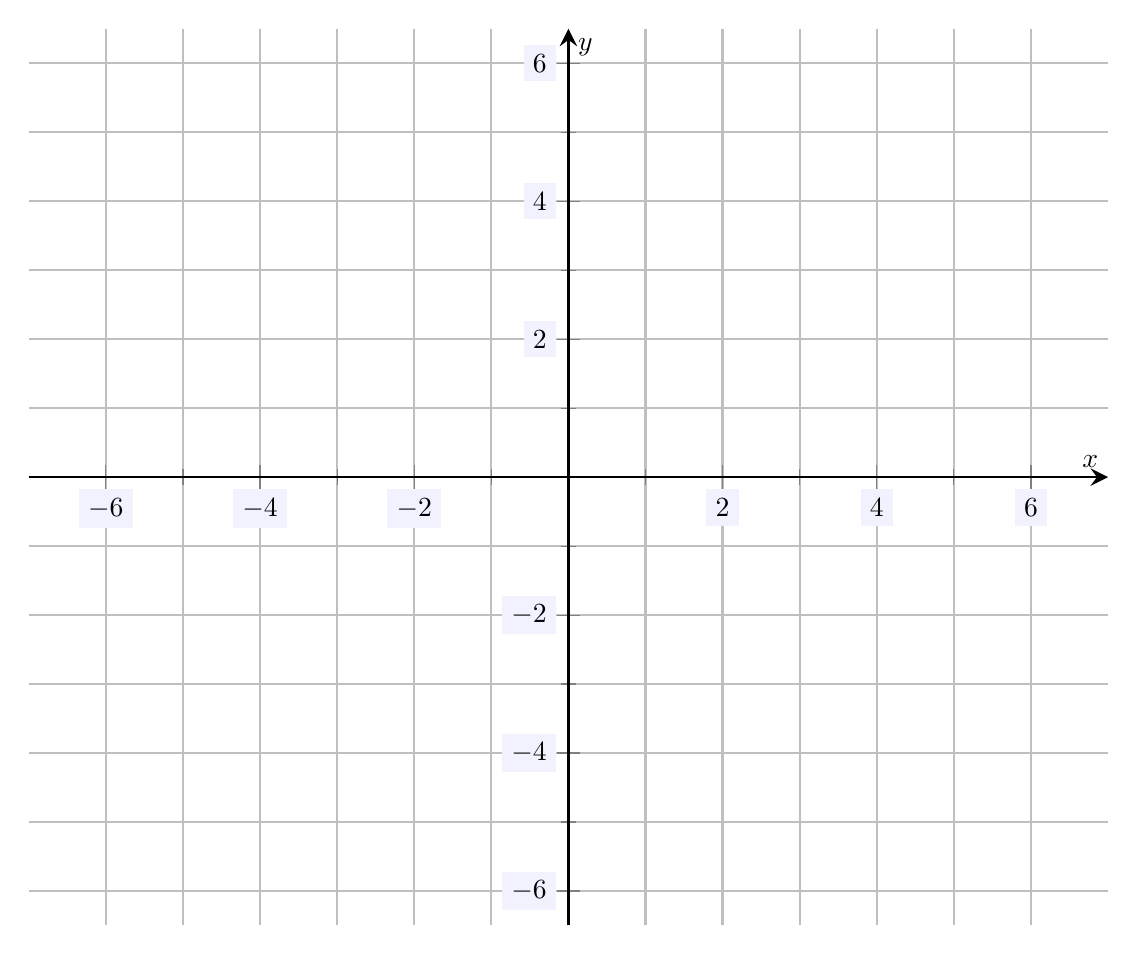
\begin{tikzpicture}[scale=2,every node/.style={scale=0.5}]
	\begin{axis}[
	grid=both,
	axis lines=middle,
	ticklabel style={fill=blue!5!white},
	xmin= -7, xmax=7,
	ymin= -6.5, ymax=6.5,
	xtick={-6,-4,-2,0,2,4,6},
	ytick={-6,-4,-2,0,2,4,6},
	minor tick = {-5,-3,...,5},
	xlabel=\(x\),ylabel=\(y\),
	]
	\end{axis}
	\end{tikzpicture}
	}
	\]



\newpage



% Problem 4
\problem{10} Plot the function $f(x):= -x^2 + 4x - 1$, being as accurate as possible. 
	\[
	\fbox{
	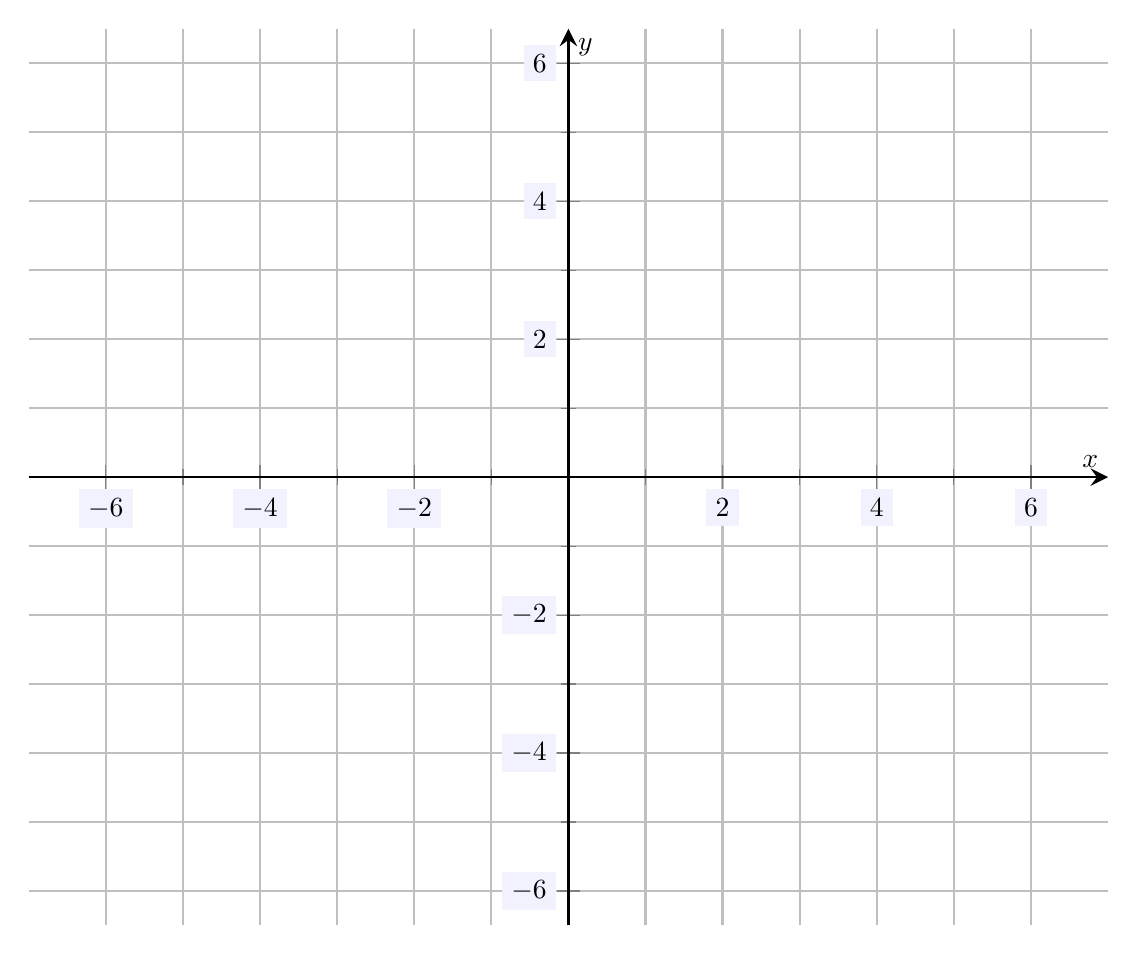
\begin{tikzpicture}[scale=2,every node/.style={scale=0.5}]
	\begin{axis}[
	grid=both,
	axis lines=middle,
	ticklabel style={fill=blue!5!white},
	xmin= -7, xmax=7,
	ymin= -6.5, ymax=6.5,
	xtick={-6,-4,-2,0,2,4,6},
	ytick={-6,-4,-2,0,2,4,6},
	minor tick = {-5,-3,...,5},
	xlabel=\(x\),ylabel=\(y\),
	]
	\end{axis}
	\end{tikzpicture}
	}
	\]


\end{document}